\section{Method}
The architecture of of our project is shown as follows. Given a software project in Java, we select the most important files as an input for extracting parsed trees in the form of ASTs. Next, we convert from tree structure of AST to sequences of AST node types. From this sequence, we transform them to a vector represented features of source code.Finally, the ML classification models will predict the range of stars for project, while the ML regression model gives developer information about actual number of stars he/she can get in the next 2 years.

\begin{figure*}
        \center{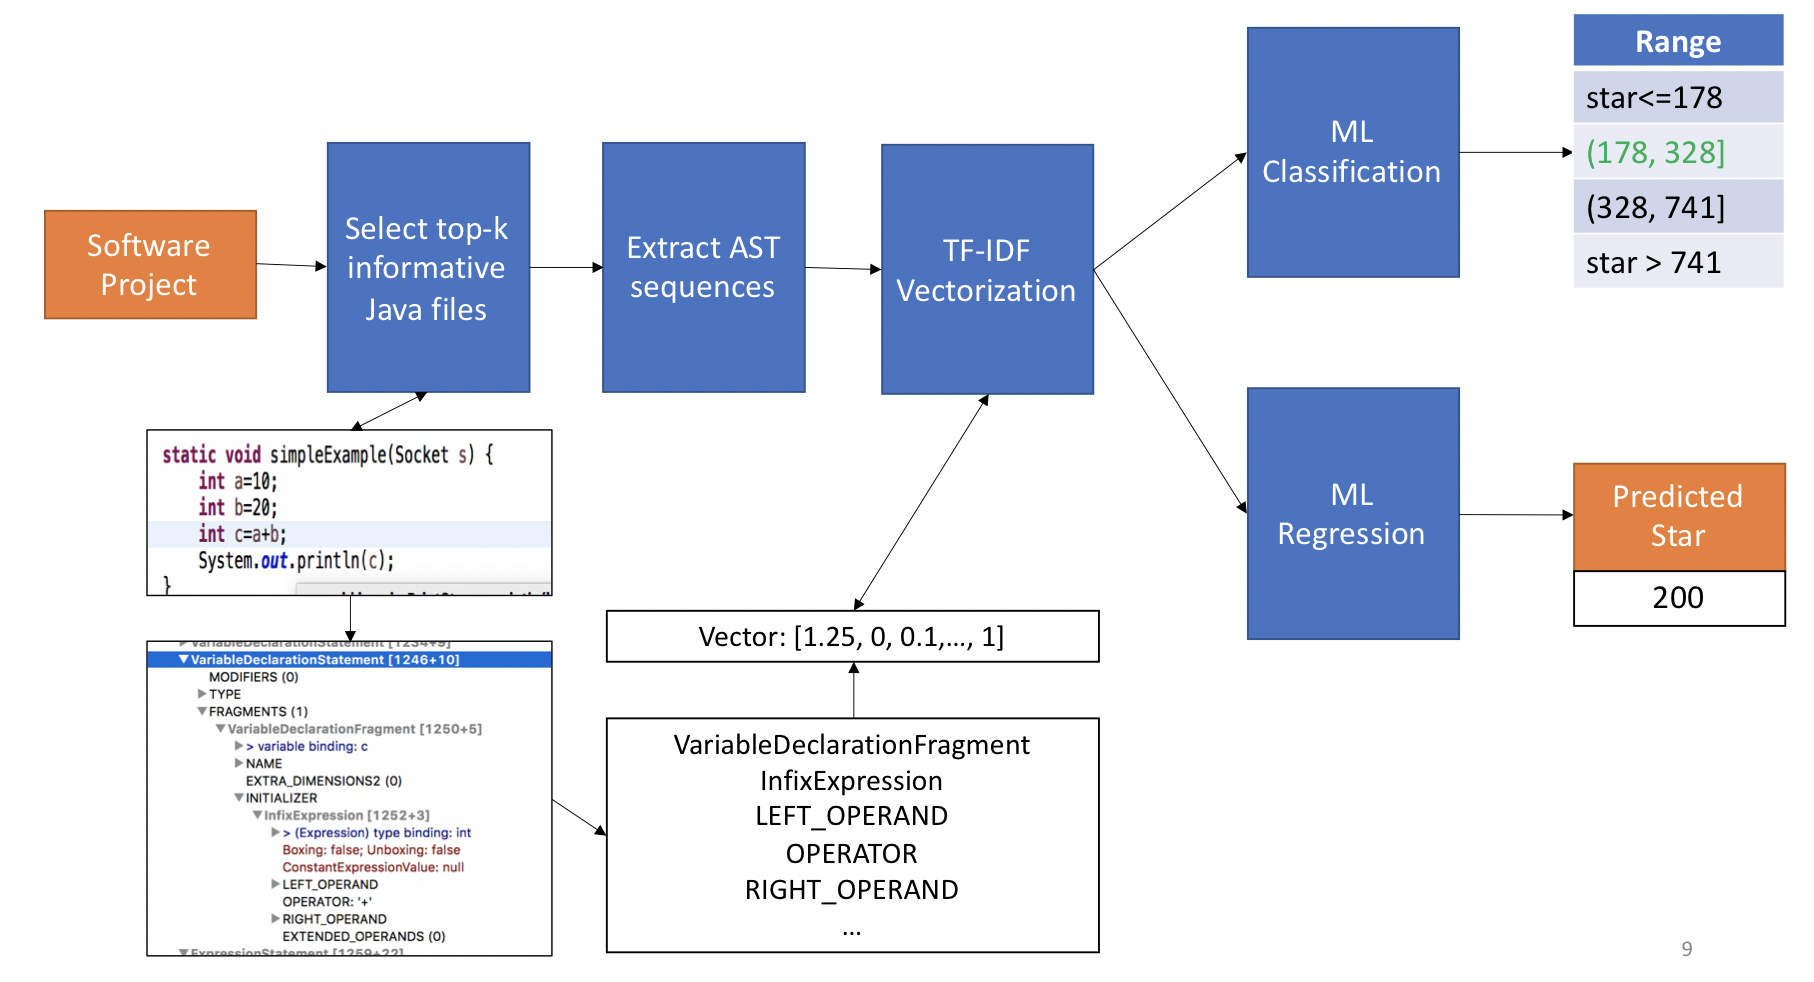
\includegraphics[width=\linewidth]
        {images/code_architecture.png}}
        \caption{Code based Github Projects Star Prediction Overview}
        \label{fig:mapping_expression} 
\end{figure*}
\subsection{Select Top-k Java Files}
The ideal solution for representing the code is to extract information about all textual files inside a Java Github project. However, this approach can be very expensive since the number of files for each industrial project can be more than 10000. More over, by experiment, we see that TF-IDF can only be scalable with small set of documents with less than 100. So, our design choice select top 50 most important files as source code. The criteria for selecting files is choosing the files with most number of \texttt{import} statements in the project. We assume that a file used multiple APIs means it is developed to solve important tasks.
\subsection{Extract AST Sequences}
Big code can contain large vocabulary \cite{015}. This fact can also bring the vectorization ended with very sparse matrix of vocabularity for each software project, which decreases the performance of TF-IDF drastically. To overcome this problem, we extract the sequence of non-terminal AST nodes instead of actual tokens. In example shows in Figure \ref{fig:mapping_expression}, we extract the AST nodes related to expression and variable declaration. The vocabulary for single word is limited to over 82 types of ASTs defined in \cite{007}.
\subsection{Range of stars for Classification}
From the training data which contained 9000 projects of \cite{013}, we select 4 ranges of stars which each range has about \texttt{25\%} of entities. The ranges of stars related to each of 4 levels is shown in Figure \ref{fig:mapping_expression}. From our obbservation, the projects with number of stars less than 178 are usually developed by independent developers, while projects with more than 741 stars are often made and maintained by big organizations.
\subsection{Optimization for TF-IDF Vectorization}
There are two strategies for making TF-IDF vectorization run efficiently in our research problem. First, we limit the n-gram to 4. This number of n-gram is the standard number used in Language Modeling in NLP problems such as in Machine Translation \cite{016}. Second, we do not use directly the feature extracted by TF-IDF. Since this approach extracts the vector with dimension equals to the size of vocabulary, the size of vector can be more than 10000. To reduce the dimension, we use Principal Component Analysis (PCA) implemented by Scikit-learn \cite{010}. 

\subsection{Hyper Parameter Tuning for Support Vector Machine Classification}
For Support Vector Machine (SVM or SVC), we care about the kernel function, which is an important configuration inside SVC. Kernel is used to transfer the data from not expected form to expected form in ML. In SVC, there are 3 types of kernels: \texttt{rbf}, \texttt{poly} and \texttt{sigmoid}. RBF, which uses Gaussian distribution, is considered as the default kernel for general purpose in SVM. Sigmoid is a function which is usually used in Neural Network but also be applicable in other ML models. Polynomial function takes advantages of polynomial variables to learn on both linear and non linear data. We will show the result of tuning kernel in the evaluation. We keep the regularization parameter \texttt{C} as 1.0 as default configuration in \cite{010}.
\subsection{Hyper Parameter Tuning for XG Boost Regression}
XGBoost Regressor is a common regression model. We select this model for tuning for regression.  We fixed the objective and column sample tree as default configuration. Based on experiences from this course, we variate the important metrics in XGBoost such as the learning rate, the max depth, the alpha and number of estimators. 


